\chapter{Effects and Animations}

Up until this chapter we have built a fully functional game that could be
shipped to the App Store! This last chapter will deal with polishing the game and making
it more delightful. \SB{} and \cocos{} provide powerful, yet simple to use tools
to create visual effects and animations. In this chapter we will add light
effects and we'll use the \SB{} timeline to bring some more motion to our
gameplay.

\section{Lighting with CCEffects}
Let's start by adding some light effects to our game. Lighting effects can make
a game feel a lot more polished. Here's a comparison of what our game looks like
right now, and how it will look once we're completed this section:

\begin{figure}[H]
    \centering
    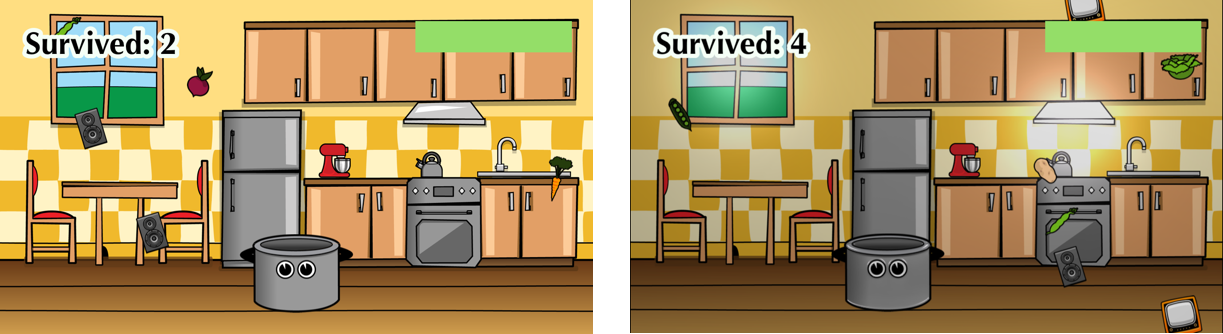
\includegraphics[width=0.9\linewidth]{images/Chapter9/lighting_comparison.png}
    \caption{Unlighted scene on the left, lighted scene on the right}
    \label{lighting_example}
\end{figure}

Most game engines require developers to write \textit{shader programs} to
use visual effects such as lighting. \cocos{} provides an API called
\inlinecode{CCEffects} that implements many common visual effects, such as
lighting, refraction, blur, etc. Using CCEffects we can enhance our games
without needing to learn how to write shader programs. 

The CCEffects can even be configured with \SB{}! We can set up all of the
lighting for this game with only a handful lines of code. 

The first step of adding lighting to our game is understanding some of the
theory that goes into lighting in 2D games.

\subsection{Lighting in 2D games}
The simplest way to light a 2D scene is to use brighter and darker colors,
depending on the distance to a given light source, I'll refer to this technique
as \textit{flat lighting}. Figure \ref{lighting_example} shows flat lighting on
the background image of our game. Some areas of the background are lighter than
others. The background is the lightest around the window and the kitchen light,
the two light sources for our game.

Flat lighting comes entirely out of the box using \cocos{}. However, using flat
lighting alone doesn't create great visual effects. In 2D games lighting can be
used to give objects a 3D feel. We are going to use that technique for the pot
and the falling objects.

We will create \textit{normal maps} for each of our game objects. A normal map
is a special kind of texture that describes the 3D surface of an object. That
way the game engine can calculate how strong certain areas of a texture should
be light up by a light source.
